\documentclass[conference]{IEEEtran}

\usepackage{amsmath}
\usepackage{amssymb}
\usepackage{graphicx}
\usepackage{booktabs}
\usepackage{xcolor}
\usepackage{colortbl}
\usepackage{cite}
\usepackage{tikz}
\usetikzlibrary{positioning, arrows.meta, calc, fit, backgrounds, decorations.pathreplacing}
\usepackage{hyperref}

\definecolor{USC_Garnet}{HTML}{73000A}
\definecolor{USC_Black10}{HTML}{ECECEC}
\definecolor{USC_Black70}{HTML}{5C5C5C}
\definecolor{USC_Congaree}{HTML}{1F414D}

\hypersetup{
  colorlinks=true,
  citecolor=USC_Garnet,
  linkcolor=USC_Garnet,
  urlcolor=USC_Congaree,
}

\title{Benchmarking Classical and Deep Learning Image Processing Methods for Object Detection in X-Band Marine Radar Imagery}

\author{
\IEEEauthorblockN{JC Vaught and Ty Dangerfield}
\IEEEauthorblockA{CSCE 763: Digital Image Processing --- Spring 2026\\
University of South Carolina\\
\{jvaught, tdangerf\}@email.sc.edu}
}

\begin{document}
\maketitle

\begin{abstract}
This project presents a systematic benchmark comparing classical digital image processing methods against modern deep learning detectors for object detection in X-band marine radar plan position indicator (PPI) imagery. On the classical side, we evaluate four CFAR detector variants (CA-, GO-, SO-, and OS-CFAR), a morphological filtering pipeline, wavelet-based detection, and Otsu thresholding with region analysis. On the deep learning side, we evaluate YOLOv11, Faster R-CNN, U-Net, and RT-DETR. All methods are tested on a shared public marine radar dataset with bounding box annotations. We stratify results by target size, range from radar, and scene density, and perform systematic failure analysis using the TIDE framework. The project directly exercises core CSCE 763 topics---image enhancement, segmentation, morphological processing, multiresolution analysis, and object recognition---while addressing an identified gap in the marine radar detection literature: the absence of a comprehensive, controlled cross-paradigm comparison.
\end{abstract}

\section{Introduction and Background}

X-band marine radar produces plan position indicator (PPI) imagery in which maritime objects---vessels, buoys, debris---appear as bright returns against sea clutter and noise. Detecting, localizing, and classifying these objects from PPI scans is a fundamental image processing problem with direct implications for maritime safety, autonomous navigation, and surveillance.

\begin{figure}[t]
\centering
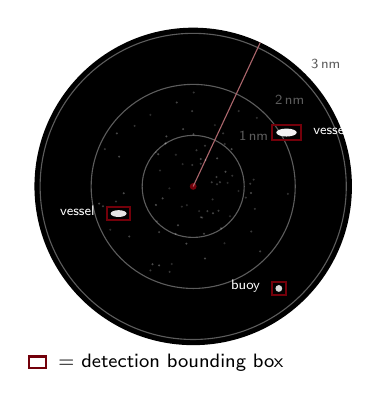
\begin{tikzpicture}[scale=0.72, every node/.style={font=\sffamily\scriptsize}]
  % Background circle (PPI display)
  \fill[black] (0,0) circle (2.8cm);
  % Range rings
  \foreach \r/\lbl in {0.9/1\,nm, 1.8/2\,nm, 2.7/3\,nm} {
    \draw[USC_Black70, thin] (0,0) circle (\r cm);
  }
  % Range ring labels
  \node[USC_Black70, anchor=south west] at (45:0.9cm) {\tiny 1\,nm};
  \node[USC_Black70, anchor=south west] at (45:1.8cm) {\tiny 2\,nm};
  \node[USC_Black70, anchor=south west] at (45:2.7cm) {\tiny 3\,nm};
  % Radar center
  \fill[USC_Garnet] (0,0) circle (0.06cm);
  % Sweep line
  \draw[USC_Garnet!60, thin] (0,0) -- (65:2.8cm);
  % Sea clutter (random dots near center)
  \pgfmathsetseed{42}
  \foreach \i in {1,...,80} {
    \pgfmathparse{rnd*1.4+0.3}\let\cR\pgfmathresult
    \pgfmathparse{rnd*360}\let\cA\pgfmathresult
    \pgfmathparse{rnd*0.15+0.15}\let\cO\pgfmathresult
    \fill[white, opacity=\cO] (\cA:\cR cm) circle (0.02cm);
  }
  % Target 1 — vessel at ~2nm, bearing 30deg
  \fill[white, opacity=0.95] (30:1.9cm) ellipse (0.18cm and 0.07cm);
  \draw[USC_Garnet, thick] ([shift={(-0.25cm,-0.13cm)}]30:1.9cm) rectangle ++(0.5cm,0.26cm);
  % Target 2 — vessel at ~1.5nm, bearing 200deg
  \fill[white, opacity=0.9] (200:1.4cm) ellipse (0.14cm and 0.06cm);
  \draw[USC_Garnet, thick] ([shift={(-0.2cm,-0.11cm)}]200:1.4cm) rectangle ++(0.4cm,0.22cm);
  % Target 3 — buoy at ~2.5nm, bearing 310deg
  \fill[white, opacity=0.85] (310:2.35cm) circle (0.06cm);
  \draw[USC_Garnet, thick] ([shift={(-0.12cm,-0.12cm)}]310:2.35cm) rectangle ++(0.24cm,0.24cm);
  % Labels
  \node[white, anchor=west, font=\sffamily\tiny] at ([shift={(0.3cm,0.05cm)}]30:1.9cm) {vessel};
  \node[white, anchor=east, font=\sffamily\tiny] at ([shift={(-0.25cm,0.05cm)}]200:1.4cm) {vessel};
  \node[white, anchor=east, font=\sffamily\tiny] at ([shift={(-0.16cm,0.05cm)}]310:2.35cm) {buoy};
  % Legend
  \draw[USC_Garnet, thick] (-2.6,-3.2) rectangle +(-0.3,0.2);
  \node[anchor=west, black] at (-2.55,-3.1) {= detection bounding box};
\end{tikzpicture}
\caption{Example PPI radar scan with annotated marine targets. Bright returns (white) represent vessels and buoys; {\color{USC_Garnet}garnet} boxes denote detection bounding boxes. Sea clutter appears as scattered low-intensity returns near the radar center.}
\label{fig:ppi_example}
\end{figure}

Classical detection approaches are rooted in core digital image processing techniques. Constant false alarm rate (CFAR) detectors~\cite{Finn1968, Rohling1983} perform adaptive \textit{image segmentation} by estimating local background statistics and thresholding accordingly. Morphological filtering~\cite{Xu2021} uses \textit{erosion, dilation, opening, and closing} to remove noise and isolate target structure. Wavelet decomposition~\cite{Duk2017} provides \textit{multiresolution analysis} to separate targets from clutter at different spatial scales. Otsu thresholding~\cite{Li2016} offers automatic \textit{image segmentation} based on histogram analysis, followed by connected component \textit{object recognition} via shape descriptors.

Recent deep learning approaches have been applied to radar PPI imagery with strong results. YOLOv11 with tiled training achieves mAP@0.5 exceeding 0.95 on the DLR DAAN dataset~\cite{Heuer2025}. Marine-Faster R-CNN reports 93.65\% recall with radar-specific architectural modifications~\cite{Chen2022}. U-Net variants have been adapted for per-pixel radar target segmentation~\cite{Onet2025}, and transformer-based detectors such as CCDN-DETR have been applied to SAR imagery~\cite{CCDNDETR2024}, though not yet to marine navigation radar. CFARnet~\cite{Diskin2024} bridges both paradigms by incorporating CFAR constraints into a deep learning loss function.

Despite these advances, \textbf{no existing study provides a comprehensive, controlled comparison of the full classical image processing pipeline against the full suite of modern deep learning detectors on a shared marine radar dataset}. Radar-PPInet~\cite{Chen2021} benchmarks only against CA-CFAR. Marine-Faster R-CNN~\cite{Chen2022} evaluates a single CFAR variant. Zhang and Li~\cite{Zhang2021} note the absence of unified evaluation criteria in their survey of deep learning for marine object detection. This project fills that gap.

\section{Connection to CSCE 763 Course Topics}

Every classical method under evaluation maps directly to a core course topic. The preprocessing stage applies \textit{image enhancement} techniques---clutter suppression, contrast adjustment, and noise reduction---to raw PPI scans before detection. The CFAR detectors and Otsu binarization perform \textit{image segmentation} by adaptively thresholding pixel intensities to separate targets from background. The morphological pipeline exercises \textit{morphological image processing} through erosion, dilation, opening, and closing operations that remove false returns and extract target structure. The wavelet-based detector demonstrates \textit{multiresolution processing} by decomposing PPI scans to analyze targets and clutter at different spatial frequency scales. Finally, shape descriptor computation and connected component classification constitute \textit{object recognition}, using area, eccentricity, and compactness to identify and characterize detected objects.

The deep learning methods are framed as learned, end-to-end extensions of these same tasks. The evaluation framework itself uses image processing metrics: intersection-over-union for localization, per-pixel segmentation accuracy for U-Net, and spatial error analysis across PPI imagery.

\begin{figure}[t]
\centering
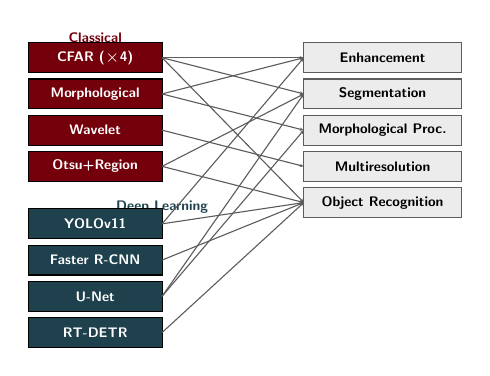
\begin{tikzpicture}[
  every node/.style={font=\sffamily\scriptsize, inner sep=2pt, outer sep=0pt},
  mnode/.style={draw, minimum height=0.38cm, minimum width=1.7cm, text=white, font=\sffamily\tiny\bfseries, anchor=west},
  cnode/.style={mnode, fill=USC_Garnet},
  dnode/.style={mnode, fill=USC_Congaree},
  tnode/.style={draw=USC_Black70, fill=USC_Black10, minimum height=0.38cm, minimum width=2.0cm, font=\sffamily\tiny\bfseries, anchor=east},
  arr/.style={-{Stealth[length=1.5pt]}, thin, USC_Black70}
]
  % Left: Methods
  \node[font=\sffamily\tiny\bfseries, USC_Garnet] at (0.85,0.25) {Classical};
  \node[cnode] (cfar) at (0,0) {CFAR ($\times$4)};
  \node[cnode, below=0.08cm of cfar] (morph) {Morphological};
  \node[cnode, below=0.08cm of morph] (wave) {Wavelet};
  \node[cnode, below=0.08cm of wave] (otsu) {Otsu+Region};

  \node[font=\sffamily\tiny\bfseries, USC_Congaree, below=0.18cm of otsu, xshift=0.85cm] {Deep Learning};
  \node[dnode, below=0.35cm of otsu] (yolo) {YOLOv11};
  \node[dnode, below=0.08cm of yolo] (frcnn) {Faster R-CNN};
  \node[dnode, below=0.08cm of frcnn] (unet) {U-Net};
  \node[dnode, below=0.08cm of unet] (rtdetr) {RT-DETR};

  % Right: Course topics
  \node[tnode] (enh) at (5.5,0) {Enhancement};
  \node[tnode, below=0.08cm of enh] (seg) {Segmentation};
  \node[tnode, below=0.08cm of seg] (morp) {Morphological Proc.};
  \node[tnode, below=0.08cm of morp] (multi) {Multiresolution};
  \node[tnode, below=0.08cm of multi] (objr) {Object Recognition};

  % Connections: Classical
  % Preprocessing (all) -> Enhancement
  \draw[arr] (cfar.east) -- (enh.west);
  \draw[arr] (morph.east) -- (enh.west);
  % CFAR -> Segmentation
  \draw[arr] (cfar.east) -- (seg.west);
  % Otsu -> Segmentation
  \draw[arr] (otsu.east) -- (seg.west);
  % Morph -> Morphological Proc
  \draw[arr] (morph.east) -- (morp.west);
  % Wavelet -> Multiresolution
  \draw[arr] (wave.east) -- (multi.west);
  % Otsu -> Object Recognition
  \draw[arr] (otsu.east) -- (objr.west);
  % CFAR -> Object Recognition (connected components)
  \draw[arr] (cfar.east) -- (objr.west);

  % Connections: Deep Learning
  \draw[arr] (yolo.east) -- (objr.west);
  \draw[arr] (frcnn.east) -- (objr.west);
  \draw[arr] (unet.east) -- (seg.west);
  \draw[arr] (rtdetr.east) -- (objr.west);
  \draw[arr] (yolo.east) -- (enh.west);
  \draw[arr] (unet.east) -- (morp.west);
\end{tikzpicture}
\caption{Mapping of each detection method to the CSCE 763 course topics it directly exercises. {\color{USC_Garnet}Classical methods} (garnet) and {\color{USC_Congaree}deep learning methods} (congaree) collectively cover all five core topics.}
\label{fig:topic_mapping}
\end{figure}

\section{Proposed Methods}

Figure~\ref{fig:pipeline} presents the complete evaluation pipeline. All 11 methods receive the same preprocessed PPI input and produce bounding box detections that feed into a unified COCO evaluation and TIDE error analysis framework.

\begin{figure*}[t]
\centering
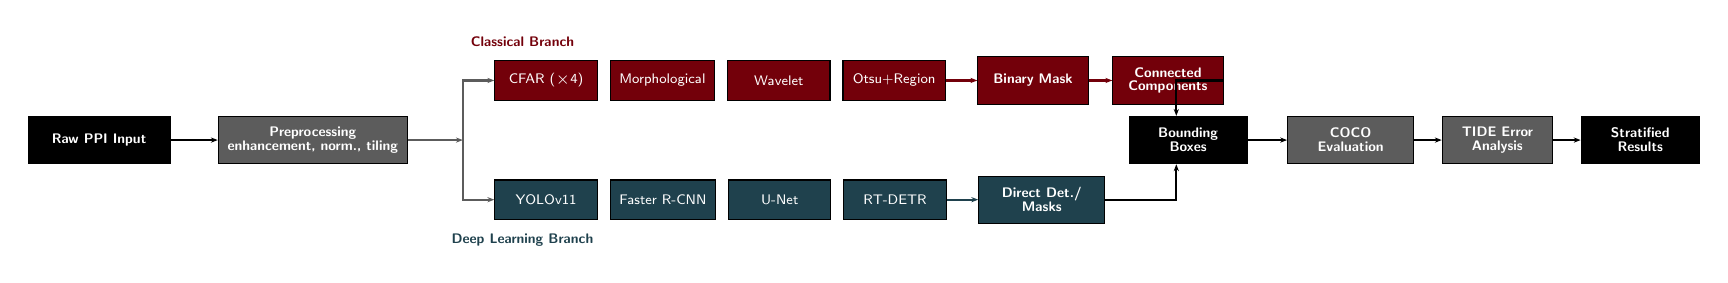
\begin{tikzpicture}[
  every node/.style={font=\sffamily\scriptsize},
  block/.style={draw, fill=#1, text=white, minimum height=0.6cm, minimum width=1.5cm, font=\sffamily\tiny\bfseries, align=center},
  block/.default={USC_Black70},
  sblock/.style={draw, fill=#1, text=white, minimum height=0.5cm, minimum width=1.3cm, font=\sffamily\tiny, align=center},
  sblock/.default={USC_Garnet},
  arr/.style={-{Stealth[length=2.5pt]}, thick},
  darr/.style={-{Stealth[length=2.5pt]}, thick, USC_Black70},
]
  % Input
  \node[block=black, minimum width=1.8cm] (input) {Raw PPI Input};

  % Preprocessing
  \node[block=USC_Black70, right=0.6cm of input, minimum width=2.2cm] (pre) {Preprocessing\\[-1pt]\tiny enhancement, norm., tiling};

  % Branch split point
  \coordinate[right=0.7cm of pre] (split);

  % Classical branch
  \node[sblock=USC_Garnet, above right=0.5cm and 0.4cm of split] (cfar) {CFAR ($\times$4)};
  \node[sblock=USC_Garnet, right=0.15cm of cfar] (morphm) {Morphological};
  \node[sblock=USC_Garnet, right=0.15cm of morphm] (wavem) {Wavelet};
  \node[sblock=USC_Garnet, right=0.15cm of wavem] (otsum) {Otsu+Region};

  % Classical intermediate
  \node[block=USC_Garnet, right=0.4cm of otsum, minimum width=1.4cm] (bmask) {Binary Mask};
  \node[block=USC_Garnet, right=0.3cm of bmask, minimum width=1.4cm] (cc) {Connected\\[-1pt]Components};

  % Deep learning branch
  \node[sblock=USC_Congaree, below right=0.5cm and 0.4cm of split] (yolo) {YOLOv11};
  \node[sblock=USC_Congaree, right=0.15cm of yolo] (frcnn) {Faster R-CNN};
  \node[sblock=USC_Congaree, right=0.15cm of frcnn] (unet) {U-Net};
  \node[sblock=USC_Congaree, right=0.15cm of unet] (rtdetr) {RT-DETR};

  % DL intermediate
  \node[block=USC_Congaree, right=0.4cm of rtdetr, minimum width=1.6cm] (direct) {Direct Det./\\[-1pt]Masks};

  % Bounding boxes (merge point)
  \coordinate[right=0.3cm of cc] (mergeTop);
  \coordinate[right=0.3cm of direct] (mergeBot);
  \coordinate (mergeC) at ($(mergeTop)!0.5!(mergeBot)$);
  \node[block=black, minimum width=1.5cm] at (mergeC) (bbox) {Bounding\\[-1pt]Boxes};

  % Evaluation
  \node[block=USC_Black70, right=0.5cm of bbox, minimum width=1.6cm] (coco) {COCO\\[-1pt]Evaluation};
  \node[block=USC_Black70, right=0.35cm of coco, minimum width=1.4cm] (tide) {TIDE Error\\[-1pt]Analysis};
  \node[block=black, right=0.35cm of tide, minimum width=1.5cm] (results) {Stratified\\[-1pt]Results};

  % Arrows
  \draw[arr] (input) -- (pre);
  \draw[darr] (pre) -- (split);
  % Split to branches
  \draw[darr] (split) |- (cfar);
  \draw[darr] (split) |- (yolo);
  % Classical chain
  \draw[arr, USC_Garnet] (otsum) -- (bmask);
  \draw[arr, USC_Garnet] (bmask) -- (cc);
  % DL chain
  \draw[arr, USC_Congaree] (rtdetr) -- (direct);
  % To bounding boxes
  \draw[arr] (cc.east) -| ([xshift=-0.15cm]bbox.north);
  \draw[arr] (direct.east) -| ([xshift=-0.15cm]bbox.south);
  % Evaluation chain
  \draw[arr] (bbox) -- (coco);
  \draw[arr] (coco) -- (tide);
  \draw[arr] (tide) -- (results);

  % Branch labels
  \node[USC_Garnet, font=\sffamily\tiny\bfseries, above=0.05cm of cfar, xshift=-0.3cm] {Classical Branch};
  \node[USC_Congaree, font=\sffamily\tiny\bfseries, below=0.05cm of yolo, xshift=-0.3cm] {Deep Learning Branch};
\end{tikzpicture}
\caption{Complete evaluation pipeline. Raw PPI scans undergo shared preprocessing before splitting into classical ({\color{USC_Garnet}garnet}) and deep learning ({\color{USC_Congaree}congaree}) branches. Both produce bounding boxes that feed into unified COCO evaluation and TIDE error analysis, enabling direct cross-paradigm comparison.}
\label{fig:pipeline}
\end{figure*}

\subsection{Classical Methods (7 total)}

\textbf{CFAR Detectors (4 variants).} We implement CA-CFAR~\cite{Finn1968}, GO-CFAR, SO-CFAR, and OS-CFAR~\cite{Rohling1983} operating on PPI imagery with 2D sliding reference windows. Guard cell size, reference cell count, and false alarm rate are tuned via grid search on a validation split. Each CFAR variant produces a binary detection mask, from which bounding boxes are extracted via connected component analysis.

\begin{figure}[t]
\centering
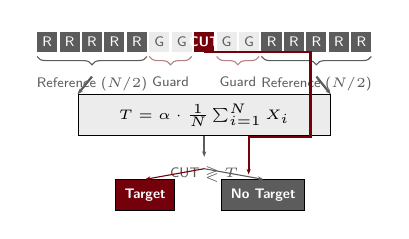
\begin{tikzpicture}[scale=0.75, every node/.style={font=\sffamily\tiny}]
  % Reference cells (left)
  \foreach \i in {0,1,2,3,4} {
    \fill[USC_Black70] (\i*0.38,0) rectangle ++(0.34,0.34);
    \node[white] at (\i*0.38+0.17,0.17) {R};
  }
  % Guard cells (left)
  \foreach \i in {5,6} {
    \fill[USC_Black10] (\i*0.38,0) rectangle ++(0.34,0.34);
    \node[USC_Black70] at (\i*0.38+0.17,0.17) {G};
  }
  % CUT
  \fill[USC_Garnet] (7*0.38,0) rectangle ++(0.34,0.34);
  \node[white, font=\sffamily\tiny\bfseries] at (7*0.38+0.17,0.17) {CUT};
  % Guard cells (right)
  \foreach \i in {8,9} {
    \fill[USC_Black10] (\i*0.38,0) rectangle ++(0.34,0.34);
    \node[USC_Black70] at (\i*0.38+0.17,0.17) {G};
  }
  % Reference cells (right)
  \foreach \i in {10,11,12,13,14} {
    \fill[USC_Black70] (\i*0.38,0) rectangle ++(0.34,0.34);
    \node[white] at (\i*0.38+0.17,0.17) {R};
  }
  % Brace under reference cells
  \draw[decorate, decoration={brace, mirror, amplitude=3pt}, USC_Black70]
    (0,-0.08) -- (4*0.38+0.34,-0.08)
    node[midway, below=4pt, USC_Black70] {Reference ($N/2$)};
  \draw[decorate, decoration={brace, mirror, amplitude=3pt}, USC_Black70]
    (10*0.38,-0.08) -- (14*0.38+0.34,-0.08)
    node[midway, below=4pt, USC_Black70] {Reference ($N/2$)};
  % Brace under guard cells
  \draw[decorate, decoration={brace, mirror, amplitude=3pt}, USC_Garnet!50]
    (5*0.38,-0.08) -- (6*0.38+0.34,-0.08)
    node[midway, below=4pt, USC_Black70] {Guard};
  \draw[decorate, decoration={brace, mirror, amplitude=3pt}, USC_Garnet!50]
    (8*0.38,-0.08) -- (9*0.38+0.34,-0.08)
    node[midway, below=4pt, USC_Black70] {Guard};
  % Arrows from reference cell regions to threshold block
  \coordinate (leftRefMid) at (2*0.38+0.17, -0.08);
  \coordinate (rightRefMid) at (12*0.38+0.17, -0.08);
  % Threshold block
  \node[draw, fill=USC_Black10, minimum height=0.45cm, minimum width=3.2cm,
        font=\sffamily\tiny, anchor=north] (thresh) at (7*0.38+0.17, -0.72)
        {$T = \alpha \cdot \frac{1}{N}\sum_{i=1}^{N} X_i$};
  \draw[-{Stealth[length=2pt]}, thick, USC_Black70] (2*0.38+0.17, -0.42) -- (thresh.north west);
  \draw[-{Stealth[length=2pt]}, thick, USC_Black70] (12*0.38+0.17, -0.42) -- (thresh.north east);
  % Arrow from threshold to comparison point
  \draw[-{Stealth[length=2pt]}, thick, USC_Black70] (thresh.south) -- ++(0,-0.35)
    node[below, font=\sffamily\tiny, USC_Black70] (comp) {CUT $\gtrless$ $T$};
  % Arrow from CUT to comparison point (routed around the right of threshold block)
  \draw[-{Stealth[length=2pt]}, thick, USC_Garnet]
    (7*0.38+0.17, 0) -- ++(1.8,0) -- ++(0,-1.45) -| (comp.east);
  % Decision outputs
  \coordinate (dec) at ($(thresh.south)+(0,-0.55)$);
  \node[draw, fill=USC_Garnet, text=white, minimum height=0.3cm,
        font=\sffamily\tiny\bfseries] (det) at ($(dec)+(-1.0,-0.45)$) {Target};
  \node[draw, fill=USC_Black70, text=white, minimum height=0.3cm,
        font=\sffamily\tiny\bfseries] (nodet) at ($(dec)+(1.0,-0.45)$) {No Target};
  \draw[-{Stealth[length=2pt]}, USC_Garnet] (dec) -- (det.north);
  \draw[-{Stealth[length=2pt]}, USC_Black70] (dec) -- (nodet.north);
\end{tikzpicture}
\caption{CA-CFAR detector sliding window architecture (1D cross-section). The cell under test (CUT) is compared against an adaptive threshold derived from surrounding reference cells.}
\label{fig:cfar_window}
\end{figure}

\textbf{Morphological Pipeline.} We apply Otsu or adaptive thresholding for initial binarization, followed by morphological opening (erosion then dilation) to remove small-scale noise, then connected component analysis with region property filtering (minimum area, eccentricity bounds) to extract target bounding boxes. Structuring element shape and size are tuned per-dataset.

\begin{figure}[t]
\centering
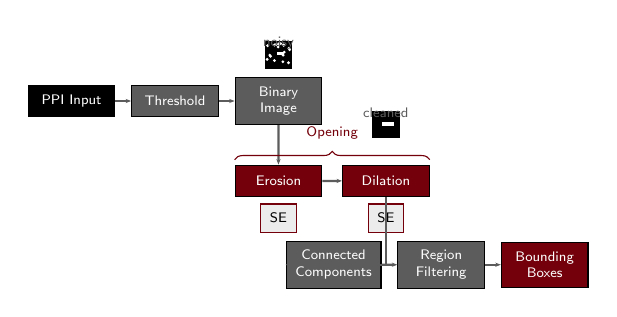
\begin{tikzpicture}[scale=0.78, every node/.style={font=\sffamily\tiny},
  block/.style={draw, fill=#1, text=white, minimum height=0.4cm,
    minimum width=1.1cm, font=\sffamily\tiny, align=center},
  block/.default={USC_Black70},
  arr/.style={-{Stealth[length=2pt]}, thick, USC_Black70},
  sebox/.style={draw=USC_Garnet, fill=USC_Black10, minimum height=0.28cm,
    minimum width=0.28cm, font=\sffamily\tiny}
]
  % Row 1
  \node[block=black] (input) {PPI Input};
  \node[block=USC_Black70, right=0.2cm of input] (otsu) {Threshold};
  \node[block=USC_Black70, right=0.2cm of otsu] (bin) {Binary\\Image};

  % Row 2 (below, shifted right)
  \node[block=USC_Garnet, below=0.5cm of bin] (ero) {Erosion};
  \node[sebox, below=0.08cm of ero] (se1) {\tiny SE};
  \node[block=USC_Garnet, right=0.25cm of ero] (dil) {Dilation};
  \node[sebox, below=0.08cm of dil] (se2) {\tiny SE};

  % Row 3 (below row 2)
  \node[block=USC_Black70, below=0.55cm of ero, xshift=0.7cm] (cc) {Connected\\Components};
  \node[block=USC_Black70, right=0.2cm of cc] (filt) {Region\\Filtering};
  \node[block=USC_Garnet, right=0.2cm of filt] (bbox) {Bounding\\Boxes};

  % Arrows row 1
  \draw[arr] (input) -- (otsu);
  \draw[arr] (otsu) -- (bin);
  % Arrow down to erosion
  \draw[arr] (bin.south) -- (ero.north);
  \draw[arr] (ero) -- (dil);
  % Opening brace over erosion+dilation pair
  \draw[decorate, decoration={brace, amplitude=3pt}, USC_Garnet]
    ([yshift=0.08cm]ero.north west) -- ([yshift=0.08cm]dil.north east)
    node[midway, above=4pt, USC_Garnet, font=\sffamily\tiny] {Opening};
  % Arrow down to CC
  \draw[arr] (dil.south) |- (cc.west);
  \draw[arr] (cc) -- (filt);
  \draw[arr] (filt) -- (bbox);

  % Illustrative before/after mini-squares
  \node[anchor=south, inner sep=0pt] at ($(bin.north)+(0,0.12)$) {%
    \tikz{
      \fill[black] (0,0) rectangle (0.35,0.35);
      \pgfmathsetseed{99}
      \foreach \i in {1,...,18} {
        \pgfmathparse{rnd*0.3+0.025}\let\px\pgfmathresult
        \pgfmathparse{rnd*0.3+0.025}\let\py\pgfmathresult
        \fill[white] (\px,\py) circle (0.02);
      }
      \fill[white] (0.15,0.18) rectangle (0.25,0.22);
    }%
  };
  \node[anchor=south, inner sep=0pt] at ($(dil.north)+(0,0.42)$) {%
    \tikz{
      \fill[black] (0,0) rectangle (0.35,0.35);
      \fill[white] (0.12,0.15) rectangle (0.28,0.21);
    }%
  };
  \node[USC_Black70, font=\sffamily\tiny] at ($(bin.north)+(0,0.55)$) {noisy};
  \node[USC_Black70, font=\sffamily\tiny] at ($(dil.north)+(0,0.85)$) {cleaned};
\end{tikzpicture}
\caption{Morphological detection pipeline. Structuring element operations remove noise before connected component extraction.}
\label{fig:morph_pipeline}
\end{figure}

\textbf{Wavelet-Based Detection.} We use the 2D stationary wavelet transform~\cite{Duk2017} to decompose PPI scans into sub-bands. Target energy concentrates in high-frequency sub-bands while clutter spreads across all bands. We threshold the detail coefficients and apply connected component extraction to produce detections.

\begin{figure}[t]
\centering
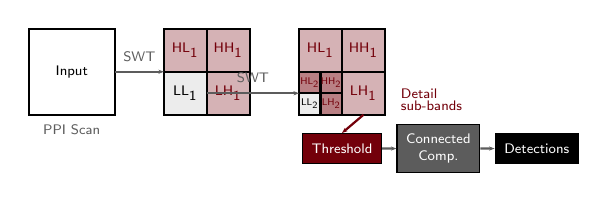
\begin{tikzpicture}[scale=0.78, every node/.style={font=\sffamily\tiny},
  arr/.style={-{Stealth[length=2pt]}, thick, USC_Black70},
  block/.style={draw, fill=#1, text=white, minimum height=0.38cm,
    minimum width=1.0cm, font=\sffamily\tiny, align=center},
  block/.default={USC_Black70}
]
  % Input image
  \draw[thick] (0,0) rectangle (1.4,1.4);
  \node at (0.7,0.7) {Input};
  \node[below, USC_Black70] at (0.7,0) {PPI Scan};

  % Level 1 decomposition
  \coordinate (l1) at (2.2,0);
  % LL1
  \draw[thick, fill=USC_Black10] (l1) rectangle ++(0.7,0.7);
  \node at ($(l1)+(0.35,0.35)$) {LL\textsubscript{1}};
  % LH1
  \draw[thick, fill=USC_Garnet!30] ($(l1)+(0.7,0)$) rectangle ++(0.7,0.7);
  \node at ($(l1)+(1.05,0.35)$) {\color{USC_Garnet}LH\textsubscript{1}};
  % HL1
  \draw[thick, fill=USC_Garnet!30] ($(l1)+(0,0.7)$) rectangle ++(0.7,0.7);
  \node at ($(l1)+(0.35,1.05)$) {\color{USC_Garnet}HL\textsubscript{1}};
  % HH1
  \draw[thick, fill=USC_Garnet!30] ($(l1)+(0.7,0.7)$) rectangle ++(0.7,0.7);
  \node at ($(l1)+(1.05,1.05)$) {\color{USC_Garnet}HH\textsubscript{1}};

  % Arrow input -> level 1
  \draw[arr] (1.4,0.7) -- (2.2,0.7) node[midway, above] {SWT};

  % Level 2 decomposition (of LL1)
  \coordinate (l2) at (4.4,0);
  % LL2
  \draw[thick, fill=USC_Black10] (l2) rectangle ++(0.35,0.35);
  \node[font=\sffamily\tiny] at ($(l2)+(0.175,0.175)$) {\scalebox{0.7}{LL\textsubscript{2}}};
  % LH2
  \draw[thick, fill=USC_Garnet!50] ($(l2)+(0.35,0)$) rectangle ++(0.35,0.35);
  \node[font=\sffamily\tiny] at ($(l2)+(0.525,0.175)$) {\scalebox{0.7}{\color{USC_Garnet}LH\textsubscript{2}}};
  % HL2
  \draw[thick, fill=USC_Garnet!50] ($(l2)+(0,0.35)$) rectangle ++(0.35,0.35);
  \node[font=\sffamily\tiny] at ($(l2)+(0.175,0.525)$) {\scalebox{0.7}{\color{USC_Garnet}HL\textsubscript{2}}};
  % HH2
  \draw[thick, fill=USC_Garnet!50] ($(l2)+(0.35,0.35)$) rectangle ++(0.35,0.35);
  \node[font=\sffamily\tiny] at ($(l2)+(0.525,0.525)$) {\scalebox{0.7}{\color{USC_Garnet}HH\textsubscript{2}}};
  % Remaining L1 detail sub-bands (right and top of L2)
  \draw[thick, fill=USC_Garnet!30] ($(l2)+(0.7,0)$) rectangle ++(0.7,0.7);
  \node at ($(l2)+(1.05,0.35)$) {\color{USC_Garnet}LH\textsubscript{1}};
  \draw[thick, fill=USC_Garnet!30] ($(l2)+(0,0.7)$) rectangle ++(0.7,0.7);
  \node at ($(l2)+(0.35,1.05)$) {\color{USC_Garnet}HL\textsubscript{1}};
  \draw[thick, fill=USC_Garnet!30] ($(l2)+(0.7,0.7)$) rectangle ++(0.7,0.7);
  \node at ($(l2)+(1.05,1.05)$) {\color{USC_Garnet}HH\textsubscript{1}};

  % Arrow LL1 -> level 2
  \draw[arr] ($(l1)+(0.7,0.35)$) -- ($(l2)+(0,0.35)$) node[midway, above] {SWT};

  % Detection pipeline below
  \node[block=USC_Garnet] (thr) at (5.1,-0.55) {Threshold};
  \node[block=USC_Black70, right=0.18cm of thr] (cc) {Connected\\Comp.};
  \node[block=black, right=0.18cm of cc] (det) {Detections};

  % Arrow from detail sub-bands down to threshold
  \draw[arr, USC_Garnet] ($(l2)+(1.05,0)$) -- (thr.north);
  \draw[arr] (thr) -- (cc);
  \draw[arr] (cc) -- (det);

  % Label for detail bands
  \node[USC_Garnet, font=\sffamily\tiny, anchor=west] at ($(l2)+(1.5,0.35)$) {Detail};
  \node[USC_Garnet, font=\sffamily\tiny, anchor=west] at ($(l2)+(1.5,0.15)$) {sub-bands};
\end{tikzpicture}
\caption{Two-level 2D wavelet decomposition (DWT layout shown for clarity; SWT preserves full spatial resolution). Target energy concentrates in detail sub-bands ({\color{USC_Garnet}garnet}), which are thresholded to produce detections.}
\label{fig:wavelet_decomp}
\end{figure}

\textbf{Otsu + Region Properties.} We apply local Otsu thresholding (SSOTSU~\cite{Li2016}) with seed-point detection to handle the small-target problem, followed by region property analysis for shape-based filtering and bounding box extraction.

\begin{figure}[t]
\centering
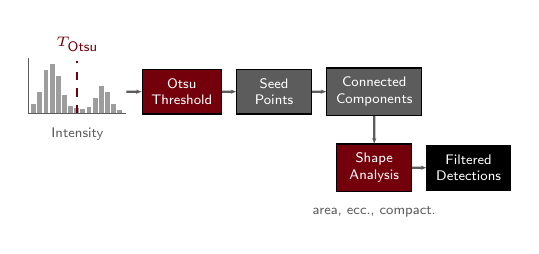
\begin{tikzpicture}[scale=0.78, every node/.style={font=\sffamily\tiny},
  block/.style={draw, fill=#1, text=white, minimum height=0.38cm,
    minimum width=0.95cm, font=\sffamily\tiny, align=center},
  block/.default={USC_Black70},
  arr/.style={-{Stealth[length=2pt]}, thick, USC_Black70}
]
  % Histogram sketch
  \begin{scope}[shift={(0,0.3)}]
    \draw[USC_Black70, thin] (0,0) -- (1.6,0); % x-axis
    \draw[USC_Black70, thin] (0,0) -- (0,0.9); % y-axis
    % Bimodal distribution bars
    \foreach \x/\h in {0.05/0.15, 0.15/0.35, 0.25/0.7, 0.35/0.8, 0.45/0.6,
                        0.55/0.3, 0.65/0.12, 0.75/0.08, 0.85/0.06,
                        0.95/0.1, 1.05/0.25, 1.15/0.45, 1.25/0.35,
                        1.35/0.15, 1.45/0.05} {
      \fill[USC_Black70, opacity=0.6] (\x,0) rectangle ++(.08,\h);
    }
    % Threshold line
    \draw[USC_Garnet, thick, dashed] (0.8,0) -- (0.8,0.85);
    \node[USC_Garnet, above, font=\sffamily\tiny] at (0.8,0.85) {$T_{\text{Otsu}}$};
    \node[below, USC_Black70] at (0.8,-0.08) {Intensity};
  \end{scope}

  % Flow blocks
  \node[block=USC_Garnet] (otsu) at (2.5,0.65) {Otsu\\Threshold};
  \node[block=USC_Black70, right=0.18cm of otsu] (seed) {Seed\\Points};
  \node[block=USC_Black70, right=0.18cm of seed] (grow) {Connected\\Components};

  % Second row
  \node[block=USC_Garnet, below=0.35cm of grow] (shape) {Shape\\Analysis};
  \node[block=black, right=0.18cm of shape] (filt) {Filtered\\Detections};

  % Shape analysis annotation
  \node[USC_Black70, font=\sffamily\tiny, below=0.06cm of shape]
    {area, ecc., compact.};

  % Arrows
  \draw[arr] (1.6,0.65) -- (otsu.west);
  \draw[arr] (otsu) -- (seed);
  \draw[arr] (seed) -- (grow);
  \draw[arr] (grow.south) -- (shape.north);
  \draw[arr] (shape) -- (filt);
\end{tikzpicture}
\caption{Otsu thresholding with region property analysis. Seed-point detection handles the small-target problem before shape-based filtering.}
\label{fig:otsu_region}
\end{figure}

\subsection{Deep Learning Methods (4 total)}

\textbf{YOLOv11} with tiled training and SAHI~\cite{Heuer2025} for sliced inference on full-resolution PPI scans. We use the oriented bounding box variant (YOLOv11-OBB) following the best-performing configuration in the literature.

\begin{figure}[t]
\centering
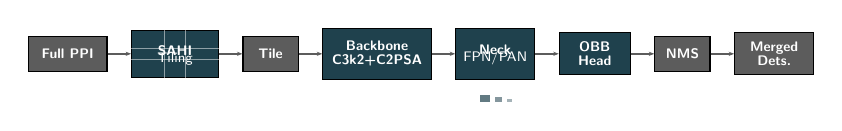
\begin{tikzpicture}[
  scale=0.72, every node/.style={font=\sffamily\tiny},
  block/.style={draw, fill=USC_Congaree, text=white, minimum height=0.45cm,
    minimum width=0.9cm, font=\sffamily\tiny\bfseries, align=center},
  nblock/.style={draw, fill=USC_Black70, text=white, minimum height=0.45cm,
    minimum width=0.9cm, font=\sffamily\tiny\bfseries, align=center},
  arr/.style={-{Stealth[length=2pt]}, thick, USC_Black70}
]
  % Full PPI image
  \node[nblock, minimum width=1.0cm] (ppi) {Full PPI};

  % SAHI Tiling block with grid overlay
  \node[block, right=0.3cm of ppi, minimum width=1.1cm, minimum height=0.6cm] (sahi) {};
  \node[font=\sffamily\tiny\bfseries, white] at ([yshift=0.05cm]sahi.center) {SAHI};
  \node[font=\sffamily\tiny, white] at ([yshift=-0.1cm]sahi.center) {Tiling};
  % Grid overlay lines inside SAHI block
  \draw[white, thin, opacity=0.5] ([xshift=-0.18cm]sahi.south) -- ([xshift=-0.18cm]sahi.north);
  \draw[white, thin, opacity=0.5] ([xshift=0.18cm]sahi.south) -- ([xshift=0.18cm]sahi.north);
  \draw[white, thin, opacity=0.5] ([yshift=-0.1cm]sahi.west) -- ([yshift=-0.1cm]sahi.east);
  \draw[white, thin, opacity=0.5] ([yshift=0.1cm]sahi.west) -- ([yshift=0.1cm]sahi.east);

  % Tile
  \node[nblock, right=0.3cm of sahi, minimum width=0.7cm] (tile) {Tile};

  % Backbone
  \node[block, right=0.3cm of tile, minimum width=1.1cm, minimum height=0.65cm] (back)
    {Backbone\\[-1pt]C3k2+C2PSA};

  % Neck with multi-scale feature visualization
  \node[block, right=0.3cm of back, minimum width=1.0cm, minimum height=0.65cm] (neck) {};
  \node[font=\sffamily\tiny\bfseries, white] at ([yshift=0.08cm]neck.center) {Neck};
  \node[font=\sffamily\tiny, white] at ([yshift=-0.08cm]neck.center) {FPN/PAN};
  % Multi-scale feature map indicators below neck
  \fill[USC_Congaree!70, draw=white, thin]
    ([yshift=-0.4cm, xshift=-0.28cm]neck.south) rectangle ++(0.2cm,0.14cm);
  \fill[USC_Congaree!55, draw=white, thin]
    ([yshift=-0.4cm, xshift=-0.02cm]neck.south) rectangle ++(0.15cm,0.11cm);
  \fill[USC_Congaree!40, draw=white, thin]
    ([yshift=-0.4cm, xshift=0.2cm]neck.south) rectangle ++(0.1cm,0.08cm);

  % OBB Head
  \node[block, right=0.3cm of neck, minimum width=0.9cm] (head) {OBB\\[-1pt]Head};

  % NMS
  \node[nblock, right=0.3cm of head, minimum width=0.7cm] (nms) {NMS};

  % Merged Detections
  \node[nblock, right=0.3cm of nms, minimum width=1.0cm] (out) {Merged\\[-1pt]Dets.};

  % Arrows
  \draw[arr] (ppi) -- (sahi);
  \draw[arr] (sahi) -- (tile);
  \draw[arr] (tile) -- (back);
  \draw[arr] (back) -- (neck);
  \draw[arr] (neck) -- (head);
  \draw[arr] (head) -- (nms);
  \draw[arr] (nms) -- (out);
\end{tikzpicture}
\caption{YOLOv11-OBB architecture with SAHI tiled inference. Full PPI scans are tiled before single-pass detection, then merged via NMS.}
\label{fig:yolov11_arch}
\end{figure}

\textbf{Faster R-CNN} with the radar-specific modifications from Marine-Faster R-CNN~\cite{Chen2022}: optimized anchor sizes for radar targets, scale normalization for range-dependent size variation, and data sampling strategies for class imbalance.

\begin{figure}[t]
\centering
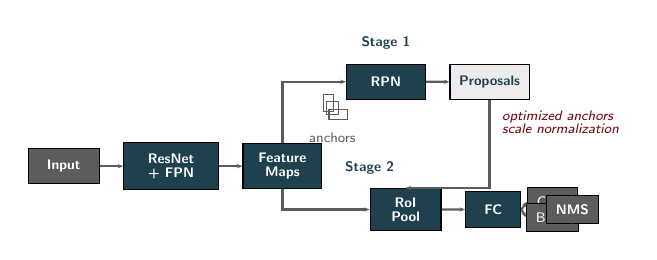
\begin{tikzpicture}[
  scale=0.72, every node/.style={font=\sffamily\tiny},
  block/.style={draw, fill=USC_Congaree, text=white, minimum height=0.45cm,
    minimum width=0.9cm, font=\sffamily\tiny\bfseries, align=center},
  nblock/.style={draw, fill=USC_Black70, text=white, minimum height=0.45cm,
    minimum width=0.9cm, font=\sffamily\tiny\bfseries, align=center},
  bgblock/.style={draw, fill=USC_Black10, minimum height=0.45cm,
    minimum width=0.9cm, font=\sffamily\tiny\bfseries, align=center,
    text=USC_Congaree},
  arr/.style={-{Stealth[length=2pt]}, thick, USC_Black70}
]
  % Input
  \node[nblock, minimum width=0.9cm] (inp) {Input};

  % Backbone
  \node[block, right=0.3cm of inp, minimum width=1.2cm, minimum height=0.6cm] (back)
    {ResNet\\[-1pt]+ FPN};

  % Feature maps
  \node[block, right=0.3cm of back, minimum width=1.0cm, minimum height=0.55cm] (feat)
    {Feature\\[-1pt]Maps};

  % Stage 1: RPN branch (above)
  \node[block, above right=0.55cm and 0.3cm of feat, minimum width=1.0cm] (rpn)
    {RPN};

  % Anchor boxes illustration near RPN
  \draw[USC_Black70, thin] ([xshift=-0.35cm, yshift=-0.25cm]rpn.south west)
    rectangle ++(0.22cm,0.22cm);
  \draw[USC_Black70, thin] ([xshift=-0.3cm, yshift=-0.35cm]rpn.south west)
    rectangle ++(0.32cm,0.18cm);
  \draw[USC_Black70, thin] ([xshift=-0.4cm, yshift=-0.2cm]rpn.south west)
    rectangle ++(0.18cm,0.3cm);
  \node[USC_Black70, font=\sffamily\tiny, anchor=north]
    at ([xshift=-0.24cm, yshift=-0.4cm]rpn.south west) {anchors};

  % Proposals
  \node[bgblock, right=0.3cm of rpn, minimum width=0.9cm] (prop) {Proposals};

  % Stage 2: RoI Pooling (below, connecting from feat and proposals)
  \node[block, right=0.6cm of feat, minimum width=0.9cm,
    yshift=-0.55cm] (roi) {RoI\\[-1pt]Pool};

  % FC Layers
  \node[block, right=0.3cm of roi, minimum width=0.7cm] (fc) {FC};

  % Classification + Box Regression outputs
  \node[nblock, minimum width=0.6cm, minimum height=0.22cm,
    font=\sffamily\tiny] (clsout) at ([yshift=0.14cm, xshift=0.55cm]fc.east) {Class};
  \node[nblock, minimum width=0.6cm, minimum height=0.22cm,
    font=\sffamily\tiny] (regout) at ([yshift=-0.14cm, xshift=0.55cm]fc.east) {BBox};

  % NMS
  \node[nblock, minimum width=0.6cm, minimum height=0.3cm] (nms)
    at ([xshift=0.9cm]fc.east) {NMS};

  % Arrows
  \draw[arr] (inp) -- (back);
  \draw[arr] (back) -- (feat);
  % Split to RPN (stage 1)
  \draw[arr] (feat.north) |- (rpn.west);
  \draw[arr] (rpn) -- (prop);
  % Proposals feed into RoI
  \draw[arr] (prop.south) |- (roi.north);
  % Feature maps also feed into RoI
  \draw[arr] (feat.south) |- (roi.west);
  \draw[arr] (roi) -- (fc);
  \draw[arr] (fc.east) -- (clsout.west);
  \draw[arr] (fc.east) -- (regout.west);
  \draw[arr] (clsout.east) -| (nms.north);
  \draw[arr] (regout.east) -| (nms.south);

  % Stage labels
  \node[USC_Congaree, font=\sffamily\tiny\bfseries, anchor=south]
    at ([yshift=0.08cm]rpn.north) {Stage 1};
  \node[USC_Congaree, font=\sffamily\tiny\bfseries, anchor=south]
    at ([yshift=0.08cm]roi.north west) {Stage 2};

  % Radar-specific annotations
  \node[USC_Garnet, font=\sffamily\tiny, anchor=west]
    at ([xshift=0.05cm, yshift=-0.3cm]prop.south) {\textit{optimized anchors}};
  \node[USC_Garnet, font=\sffamily\tiny, anchor=west]
    at ([xshift=0.05cm, yshift=-0.5cm]prop.south) {\textit{scale normalization}};
\end{tikzpicture}
\caption{Faster R-CNN two-stage architecture with radar-specific anchor optimization and scale normalization for range-dependent target size variation.}
\label{fig:frcnn_arch}
\end{figure}

\textbf{U-Net} for per-pixel semantic segmentation of radar returns, producing target masks from which bounding boxes are derived. This provides an alternative detection paradigm (segmentation-based vs. box regression).

\begin{figure}[t]
\centering
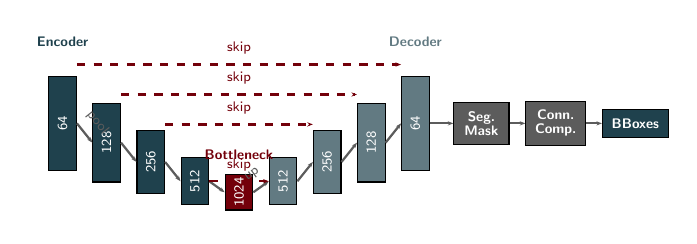
\begin{tikzpicture}[
  scale=0.7, every node/.style={font=\sffamily\tiny},
  enc/.style={draw, fill=USC_Congaree, text=white, minimum width=0.35cm,
    font=\sffamily\tiny\bfseries, align=center},
  dec/.style={draw, fill=USC_Congaree!70, text=white, minimum width=0.35cm,
    font=\sffamily\tiny\bfseries, align=center},
  nblock/.style={draw, fill=USC_Black70, text=white, minimum height=0.35cm,
    minimum width=0.7cm, font=\sffamily\tiny\bfseries, align=center},
  arr/.style={-{Stealth[length=2pt]}, thick, USC_Black70},
  skip/.style={-{Stealth[length=2pt]}, thick, USC_Garnet, dashed}
]
  % Encoder path (left side, going down)
  \node[enc, minimum height=1.2cm] (e1) at (0, 0) {};
  \node[enc, minimum height=1.0cm] (e2) at (0.8, -0.35) {};
  \node[enc, minimum height=0.8cm] (e3) at (1.6, -0.7) {};
  \node[enc, minimum height=0.6cm] (e4) at (2.4, -1.05) {};

  % Bottleneck
  \node[draw, fill=USC_Garnet, text=white, minimum height=0.45cm,
    minimum width=0.35cm, font=\sffamily\tiny\bfseries] (bn) at (3.2, -1.25) {};

  % Decoder path (right side, going up)
  \node[dec, minimum height=0.6cm] (d4) at (4.0, -1.05) {};
  \node[dec, minimum height=0.8cm] (d3) at (4.8, -0.7) {};
  \node[dec, minimum height=1.0cm] (d2) at (5.6, -0.35) {};
  \node[dec, minimum height=1.2cm] (d1) at (6.4, 0) {};

  % Labels on blocks
  \node[white, rotate=90, font=\sffamily\tiny] at (e1) {64};
  \node[white, rotate=90, font=\sffamily\tiny] at (e2) {128};
  \node[white, rotate=90, font=\sffamily\tiny] at (e3) {256};
  \node[white, rotate=90, font=\sffamily\tiny] at (e4) {512};
  \node[white, rotate=90, font=\sffamily\tiny] at (bn) {1024};
  \node[white, rotate=90, font=\sffamily\tiny] at (d4) {512};
  \node[white, rotate=90, font=\sffamily\tiny] at (d3) {256};
  \node[white, rotate=90, font=\sffamily\tiny] at (d2) {128};
  \node[white, rotate=90, font=\sffamily\tiny] at (d1) {64};

  % Encoder arrows (conv + pool, going down)
  \draw[arr] (e1.east) -- (e2.west) node[midway, above, sloped, font=\sffamily\tiny] {pool};
  \draw[arr] (e2.east) -- (e3.west);
  \draw[arr] (e3.east) -- (e4.west);
  \draw[arr] (e4.east) -- (bn.west);

  % Decoder arrows (upconv, going up)
  \draw[arr] (bn.east) -- (d4.west) node[midway, above, sloped, font=\sffamily\tiny] {up};
  \draw[arr] (d4.east) -- (d3.west);
  \draw[arr] (d3.east) -- (d2.west);
  \draw[arr] (d2.east) -- (d1.west);

  % Skip connections (horizontal dashed arrows)
  \draw[skip] (e4.east |- d4.west) -- (d4.west)
    node[midway, above, font=\sffamily\tiny, USC_Garnet] {skip};
  \draw[skip] ([yshift=0.1cm]e3.north east) -- ([yshift=0.1cm]d3.north west)
    node[midway, above, font=\sffamily\tiny, USC_Garnet] {skip};
  \draw[skip] ([yshift=0.15cm]e2.north east) -- ([yshift=0.15cm]d2.north west)
    node[midway, above, font=\sffamily\tiny, USC_Garnet] {skip};
  \draw[skip] ([yshift=0.2cm]e1.north east) -- ([yshift=0.2cm]d1.north west)
    node[midway, above, font=\sffamily\tiny, USC_Garnet] {skip};

  % Output: segmentation mask -> connected components -> bounding boxes
  \node[nblock, right=0.3cm of d1] (mask) {Seg.\\[-1pt]Mask};
  \node[nblock, right=0.2cm of mask] (cc) {Conn.\\[-1pt]Comp.};
  \node[draw, fill=USC_Congaree, text=white, minimum height=0.35cm,
    minimum width=0.7cm, font=\sffamily\tiny\bfseries, right=0.2cm of cc] (bbx) {BBoxes};

  \draw[arr] (d1.east) -- (mask.west);
  \draw[arr] (mask) -- (cc);
  \draw[arr] (cc) -- (bbx);

  % Section labels
  \node[USC_Congaree, font=\sffamily\tiny\bfseries, anchor=south] at ([yshift=0.35cm]e1.north) {Encoder};
  \node[USC_Garnet, font=\sffamily\tiny\bfseries, anchor=south] at ([yshift=0.08cm]bn.north) {Bottleneck};
  \node[USC_Congaree!70, font=\sffamily\tiny\bfseries, anchor=south] at ([yshift=0.35cm]d1.north) {Decoder};
\end{tikzpicture}
\caption{U-Net encoder-decoder architecture with skip connections for per-pixel radar target segmentation.}
\label{fig:unet_arch}
\end{figure}

\textbf{RT-DETR} as a transformer-based, end-to-end detector. This architecture has not been applied to marine radar PPI imagery in the literature, representing a novel baseline contribution.

\begin{figure}[t]
\centering
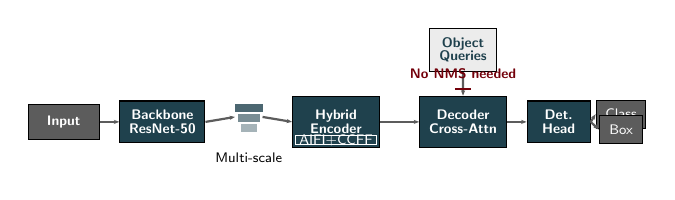
\begin{tikzpicture}[
  scale=0.7, every node/.style={font=\sffamily\tiny},
  block/.style={draw, fill=USC_Congaree, text=white, minimum height=0.45cm,
    minimum width=0.85cm, font=\sffamily\tiny\bfseries, align=center},
  nblock/.style={draw, fill=USC_Black70, text=white, minimum height=0.45cm,
    minimum width=0.85cm, font=\sffamily\tiny\bfseries, align=center},
  bgblock/.style={draw, fill=USC_Black10, minimum height=0.45cm,
    minimum width=0.85cm, font=\sffamily\tiny\bfseries, align=center,
    text=USC_Congaree},
  arr/.style={-{Stealth[length=2pt]}, thick, USC_Black70}
]
  % Input
  \node[nblock, minimum width=0.9cm] (inp) {Input};

  % Backbone
  \node[block, right=0.25cm of inp, minimum width=1.0cm] (back) {Backbone\\[-1pt]ResNet-50};

  % Multi-scale features (three stacked rectangles)
  \coordinate[right=0.55cm of back] (msc);
  \fill[USC_Congaree!80] ([yshift=0.18cm, xshift=-0.25cm]msc) rectangle ++(0.5cm,0.14cm);
  \fill[USC_Congaree!60] ([yshift=0.0cm, xshift=-0.2cm]msc) rectangle ++(0.4cm,0.14cm);
  \fill[USC_Congaree!40] ([yshift=-0.18cm, xshift=-0.15cm]msc) rectangle ++(0.3cm,0.14cm);
  \node[font=\sffamily\tiny, anchor=north] at ([yshift=-0.38cm]msc) {Multi-scale};

  % Hybrid Encoder
  \node[block, right=0.55cm of msc, minimum width=1.1cm, minimum height=0.65cm] (enc) {Hybrid\\[-1pt]Encoder};
  % Self-attention label inside encoder
  \draw[white, thin] ([yshift=0.06cm, xshift=0.06cm]enc.south west)
    rectangle ([yshift=0.22cm, xshift=-0.06cm]enc.south east);
  \node[white, font=\sffamily\tiny] at ([yshift=0.14cm]enc.south) {AIFI+CCFF};

  % Transformer Decoder
  \node[block, right=0.5cm of enc, minimum width=1.1cm, minimum height=0.65cm] (dec) {Decoder\\[-1pt]Cross-Attn};

  % Object Queries (parallel input from above)
  \node[bgblock, above=0.3cm of dec, minimum width=0.85cm] (oq) {Object\\[-1pt]Queries};

  % Detection Head
  \node[block, right=0.25cm of dec, minimum width=0.8cm] (head) {Det.\\[-1pt]Head};

  % Outputs (class + box)
  \node[nblock, minimum width=0.55cm, minimum height=0.22cm,
    font=\sffamily\tiny] (cls) at ([yshift=0.14cm, xshift=0.55cm]head.east) {Class};
  \node[nblock, minimum width=0.55cm, minimum height=0.22cm,
    font=\sffamily\tiny] (box) at ([yshift=-0.14cm, xshift=0.55cm]head.east) {Box};

  % Arrows
  \draw[arr] (inp) -- (back);
  \draw[arr] (back.east) -- ([xshift=-0.25cm, yshift=0.09cm]msc);
  \draw[arr] ([xshift=0.25cm, yshift=0.09cm]msc) -- (enc.west);
  \draw[arr] (enc) -- (dec);
  \draw[arr] (oq.south) -- (dec.north);
  \draw[arr] (dec) -- (head);
  \draw[arr] (head.east) -- (cls.west);
  \draw[arr] (head.east) -- (box.west);

  % "No NMS" annotation
  \draw[USC_Garnet, thick] ([yshift=0.12cm, xshift=-0.15cm]dec.north) --
    ([yshift=0.12cm, xshift=0.15cm]dec.north);
  \node[USC_Garnet, font=\sffamily\tiny\bfseries, anchor=south]
    at ([yshift=0.14cm]dec.north) {No NMS needed};
\end{tikzpicture}
\caption{RT-DETR transformer-based detector. End-to-end detection without NMS post-processing via learned object queries and cross-attention decoding.}
\label{fig:rtdetr_arch}
\end{figure}

\section{Evaluation Plan}

\subsection{Dataset}

We will use the DLR DAAN dataset~\cite{Heuer2025}, which provides 760 full-resolution X-band marine radar PPI frames with bounding box, oriented bounding box, and instance segmentation annotations. When tiled at 640$\times$640, this yields 3,040 training images with 11,893 labeled instances. We split temporally (by recording session, not by frame) to prevent data leakage from correlated scans.

\subsection{Metrics}

We adopt the COCO evaluation protocol: AP@0.5, AP@0.75, AP@[0.50:0.95], AR@1, AR@10, AR@100, stratified by object size (AP\textsubscript{S}, AP\textsubscript{M}, AP\textsubscript{L}). For classical methods producing binary masks, we convert to bounding boxes via connected components before evaluation. We also report inference time (ms/frame), FLOPs, and parameter count for computational comparison.

\subsection{Failure Analysis}

We apply the TIDE framework~\cite{Bolya2020} to decompose each method's errors into classification, localization, duplicate, background, and missed detection components. We additionally stratify performance by range from radar center, target density per scan, and target size in pixels to identify condition-dependent failure modes.

\subsection{Statistical Rigor}

Deep learning models are trained with 3 random seeds; we report mean and standard deviation. Pairwise method comparisons use paired bootstrap testing (10,000 resamples) with Bonferroni correction. We give equal hyperparameter tuning effort to classical and deep learning methods to ensure fairness.

% --- Full-width table spanning both columns ---
\begin{table*}[t]
\centering
\caption{Project Timeline and Division of Responsibilities}
\vspace{0.3em}
\renewcommand{\arraystretch}{1.2}
\begin{tabular}{@{} >{\bfseries}c p{5.8cm} p{5.8cm} p{2.4cm} @{}}
\toprule
\rowcolor{USC_Black10} \textbf{Week} & \textbf{JC Vaught} & \textbf{Ty Dangerfield} & \textbf{Milestone} \\
\midrule
1--2 & Download DLR DAAN dataset; implement PPI preprocessing pipeline (polar-to-Cartesian, normalization, tiling) & Set up training infrastructure (GPU environment, data loaders, COCO-format annotation conversion) & Data ready \\
\rowcolor{USC_Black10}
3--5 & Implement CA-CFAR, GO-CFAR, SO-CFAR, OS-CFAR with 2D sliding windows; implement morphological pipeline, wavelet detection, and Otsu+regionprops & Train YOLOv11-OBB with SAHI, Faster R-CNN with radar modifications, U-Net segmentation, and RT-DETR; tune hyperparameters on validation split & All methods implemented \\
5--7 & Run classical methods across full test set; tune CFAR parameters (guard cells, reference cells, $P_{FA}$) and morphological structuring elements & Run deep learning inference across test set with 3 seeds per model; collect per-image predictions in COCO format & Raw results collected \\
\rowcolor{USC_Black10}
7--8 & Run TIDE error analysis on all methods; build stratified evaluation (by range, size, density); generate failure case visualizations & Measure inference time, FLOPs, parameter counts; build Pareto plots (accuracy vs. speed); run paired bootstrap significance tests & Analysis complete \\
9 & Write Introduction, Background, Classical Methods, and Failure Analysis sections of final report & Write Deep Learning Methods, Evaluation, and Results sections; prepare presentation slides & Report and presentation ready \\
\bottomrule
\end{tabular}
\vspace{0.3em}
\noindent\small\textit{Note: Week 4 (Mar 8--15) is spring break. Nine working weeks total from Feb 17 through Apr 27.}
\end{table*}

\section{Expected Contributions}

This project will produce three outputs. First, the first comprehensive cross-paradigm benchmark for marine radar PPI object detection, comparing 7 classical and 4 deep learning methods under identical conditions. Second, a systematic failure analysis revealing when and why each paradigm fails, providing actionable guidance for practitioners selecting detection methods. Third, a computational efficiency analysis via Pareto plots showing the accuracy-latency tradeoff, which is critical for real-time maritime applications where X-band radar rotates at 20--25 RPM (one scan every 2.4--3 seconds).

\bibliographystyle{IEEEtran}
\begin{thebibliography}{13}

\bibitem{Finn1968} H.~M. Finn and R.~S. Johnson, ``Adaptive detection mode with threshold control as a function of spatially sampled clutter-level estimates,'' \textit{RCA Review}, vol.~29, no.~9, pp.~414--464, 1968.

\bibitem{Rohling1983} H.~Rohling, ``Radar CFAR thresholding in clutter and multiple target situations,'' \textit{IEEE Trans. Aerosp. Electron. Syst.}, vol.~AES-19, no.~4, pp.~608--621, 1983.

\bibitem{Duk2017} V.~Duk, L.~Rosenberg, and B.~W.-H. Ng, ``Target detection in sea-clutter using stationary wavelet transforms,'' \textit{IEEE Trans. Aerosp. Electron. Syst.}, vol.~53, no.~3, pp.~1136--1146, 2017.

\bibitem{Li2016} Q.~Li \textit{et al.}, ``A speed-up seed point Otsu method for ship detection in various scenarios,'' in \textit{Proc. IEEE IGARSS}, 2016, pp.~6421--6424.

\bibitem{Xu2021} Y.~Xu \textit{et al.}, ``Adaptive clustering-based marine radar sea clutter normalization,'' \textit{J. Sensors}, vol.~2021, Art.~2938251, 2021.

\bibitem{Chen2021} X.~Chen \textit{et al.}, ``Multi-dimensional automatic detection of scanning radar images of marine targets based on Radar PPInet,'' \textit{Remote Sensing}, vol.~13, no.~19, Art.~3856, 2021.

\bibitem{Chen2022} X.~Chen \textit{et al.}, ``Marine target detection based on Marine-Faster R-CNN for navigation radar PPI images,'' \textit{Front. Inf. Technol. Electron. Eng.}, vol.~23, 2022.

\bibitem{Heuer2025} M.~Heuer \textit{et al.}, ``High-precision marine radar object detection using tiled training and SAHI enhanced YOLOv11-OBB,'' \textit{Sensors}, vol.~26, no.~3, Art.~942, 2025.

\bibitem{Onet2025} J.~Yee, ``Onet: Twin U-Net architecture for unsupervised binary semantic segmentation in radar and remote sensing images,'' \textit{IEEE Trans. Image Process.}, 2025.

\bibitem{CCDNDETR2024} L.~Zhang \textit{et al.}, ``CCDN-DETR: A detection transformer based on constrained contrast denoising for multi-class SAR object detection,'' \textit{Sensors}, vol.~24, no.~6, Art.~1793, 2024.

\bibitem{Diskin2024} T.~Diskin \textit{et al.}, ``CFARnet: Deep learning for target detection with constant false alarm rate,'' \textit{Signal Process.}, vol.~223, Art.~109543, 2024.

\bibitem{Bolya2020} D.~Bolya \textit{et al.}, ``TIDE: A general toolbox for identifying object detection errors,'' in \textit{Proc. ECCV}, 2020.

\bibitem{Zhang2021} X.~Zhang and X.~Li, ``Survey on deep learning-based marine object detection,'' \textit{J. Adv. Transp.}, vol.~2021, Art.~5808206, 2021.

\end{thebibliography}

\end{document}
